\section{Dataset}

\begin{frame}{Dataset}

    Direct use of tax data is restricted due to privacy concerns, so we rely on a proxy dataset for our case study.\\
  

    \visible<2->{Requirements for the proxy dataset:}
    \begin{itemize}
        \item<3-> Dataset heterogeneity
        \item<4-> Structured hierarchy
    \end{itemize}
\end{frame}


\begin{frame}{\ac{dataset}\footnote{\url{https://archive.org/details/ETYNTKE} (29.01.2025)}}
    \begin{columns}[T] % align top
        \begin{column}{0.6\textwidth}
             \begin{itemize}
                \item $\approx 101$ GB 
                \item Images, text documents, and other file types
                \item Malformed files
                \item Uploaded in 2015
                \item Topics include politics, weaponry, and computer science
                \item Hierarchical organization into directories
            \end{itemize}
        \end{column}

        \begin{column}{0.25\textwidth}
            \begin{figure}
                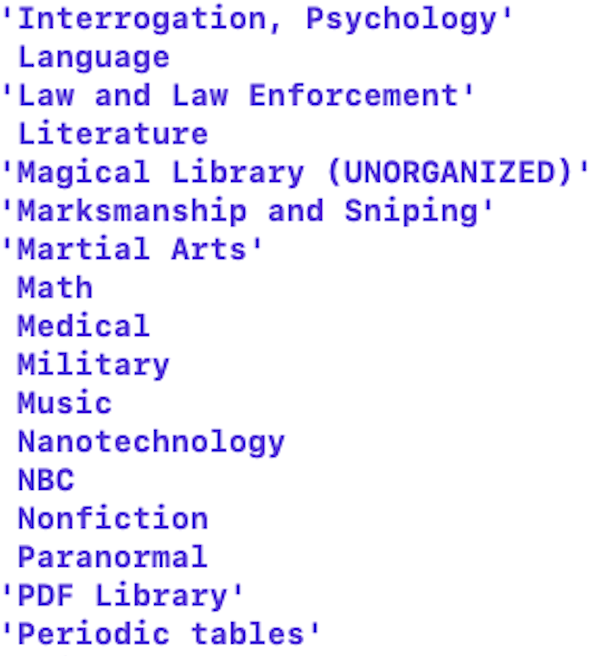
\includegraphics[width=\linewidth]{images/screenshot_data.png}
                \caption{Subset of top-level directories.} % replaces \caption
            \end{figure}
   
        \end{column}
    \end{columns}
\end{frame}
